%!TEX root=../master_thesis.tex
\chapter{Components}
\label{chap:components}
In this chapter all modules Riak Core Lite consists of are listed, shortly described, and grouped into logical components.
A visual overview of the components can be found in Figure \ref{fig:components}.
Modules relevant to this thesis 
\begin{figure}
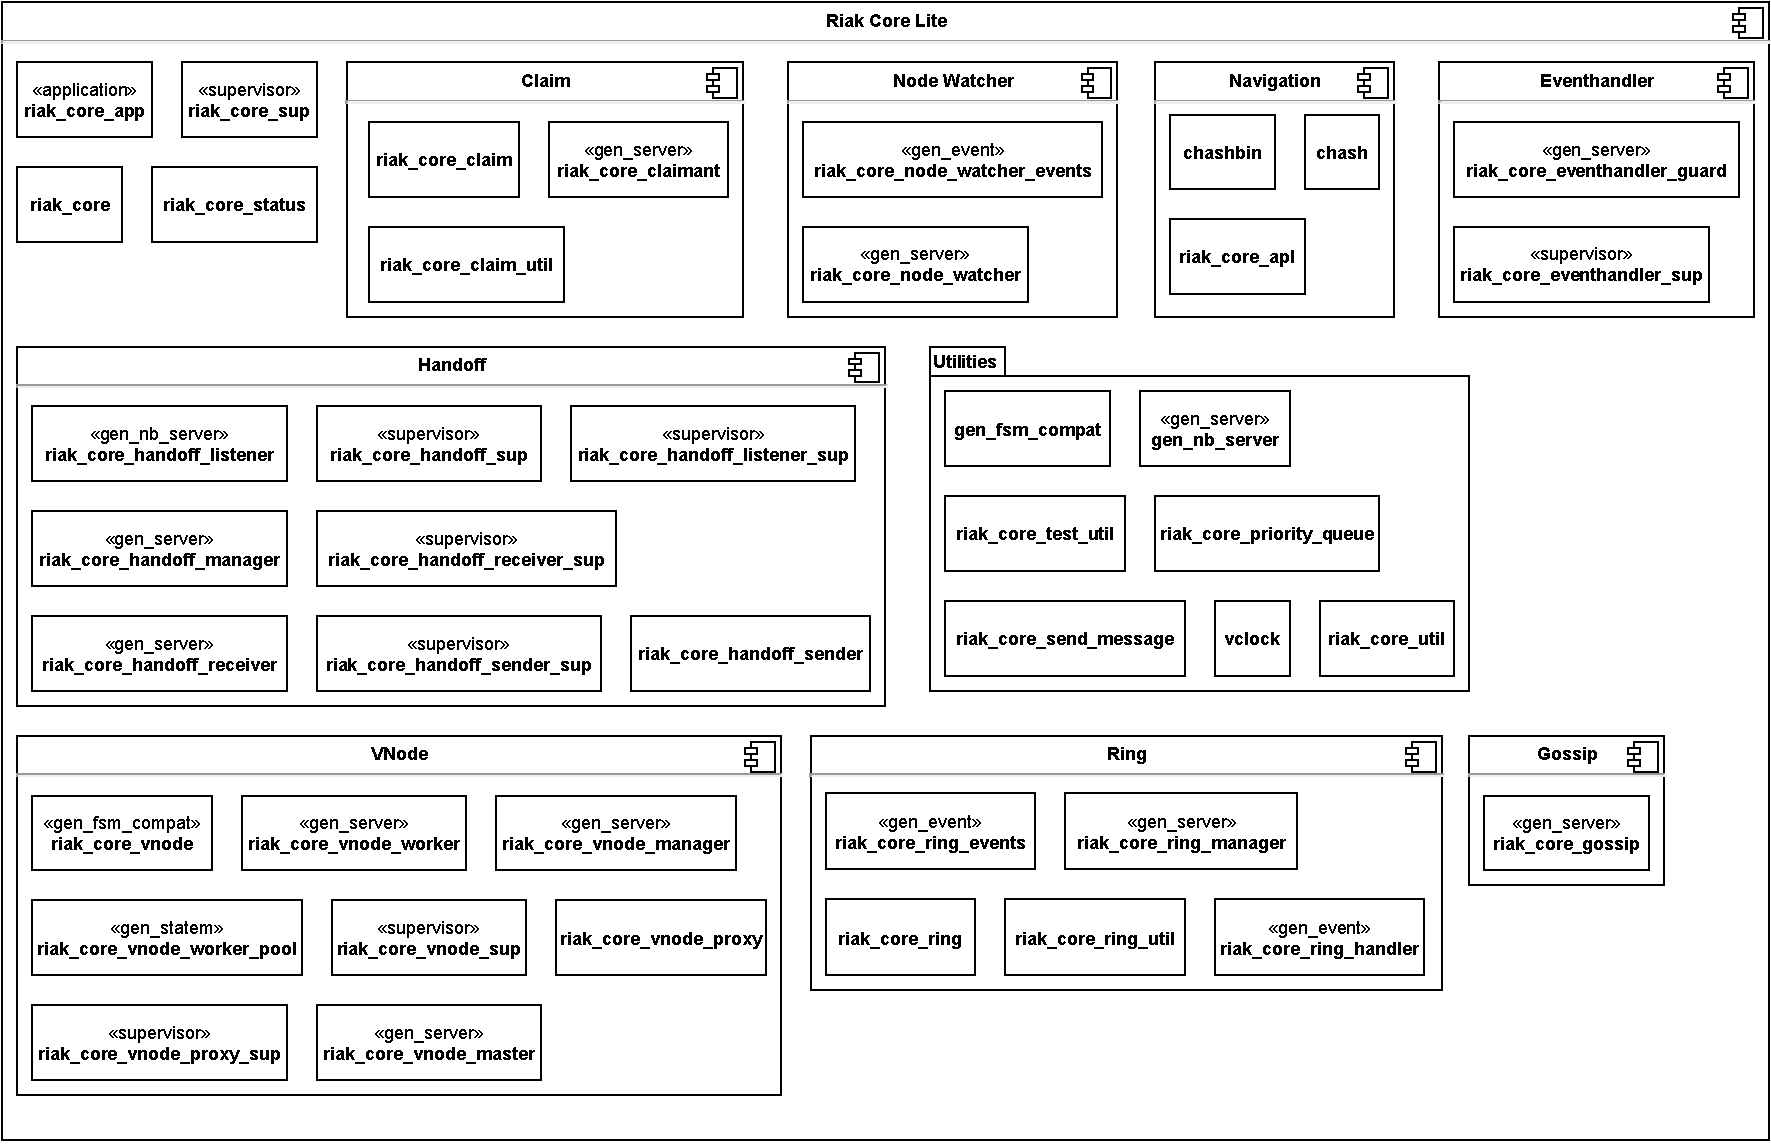
\includegraphics[width=\textwidth]{components}
\caption[System Components]{System Components. Multiple system modules are grouped into logical components to make a superficient description possible.}
\label{fig:components}
\end{figure}

\section{Top Level Modules}
	Top level modules are modules that cannot be assigned to a logical component as their responsibilities lie within a global scope with regard to the system.
	\subsection{riak\_core\_app}
		This module is the entry point to start and stop a system instance.
	
	\subsection{riak\_core\_sup}
		This module is the root Riak Core Lite's supervisor tree and is responsible to keep the system running.
		It exclusively supervises other more specific supervisors.
	
	\subsection{riak\_core}
		The \lstinline!riak_core! module wraps most of the system's core functionality like adding and removing nodes or register applications using the Riak Core instance as a backend.
	
	\subsection{riak\_core\_status}
		This module provides functions to check different information of the system such as the status of the ring or ongoing and scheduled transfers.


\section{Claim}
	In Riak Core Lite the claim system is responsible for managing the ring configuration and updating the ring at appropriate times.
	\subsection{riak\_core\_claim}
		The claim modules implements the claim algorithm.
		This algorithm determines the assignment of sections of the ring to owner nodes such that a sufficiently good load balancing is achieved.
	
	\subsection{riak\_core\_claimant}
		The claimant module is responsible for planning and triggering changes to the cluster and ring.
		There is exactly one claimant service at a time responsible for one ring.
		However, the claimant may change while the system is running.
		The claimant works with a stage-plan-commit model in which first a number of changes like adding nodes or resizing the ring are scheduled for the current claimant.
		Before committing these changes a plan showing the impact of applying those changes.
		When committed, changes are applied to the current ring.
		The claimant is also responsible for deciding when to install the updated ring.
	
	\subsection{riak\_core\_claim\_util}
		This module is a library of utility functions linked to the claim algorithm.

\section{Node Watcher}
	The node watcher component groups components that are responsible for the health of nodes.
	\subsection{riak\_core\_node\_watcher\_events}
		This module allows for event handling implementations for events concerning the health of nodes.
		This can be used to handle a high work load or connectivity issues.
	
	\subsection{riak\_core\_node\_watcher}
		The node watcher provides an interface to retrieve information about the current node health.
	

\section{Navigation}
	The navigation component contains modules concerning the placement of nodes on the ring and replicas on the nodes.
	\subsection{riak\_core\_chashbin}
		This module provides a library to work with a binary encoding of a Consistent Hashing structure that can be used for faster access times.
		The library provides read-only functionality and is mostly used to compute preference lists.
	
	\subsection{riak\_core\_chash}
		A library providing functions to work with a Consistent Hashing structure.
		It can be used to manipulate a structure and access information about the structure.
		The structure stores information of section ownership and is the base for the ring structure.
	
	\subsection{riak\_core\_apl}
		The module \lstinline!riak_core_apl!'s name is short for active preference list.
		It is the entry point to query the system for a preference list containing only nodes that are seen as active by the cluster.
		There are different variants of annotations and filters one can choose to retrieve together with the preference list. 
	

\section{Eventhandler}
	The event handler component contains modules providing utilities for event handlers.
	\subsection{riak\_core\_eventhandler\_guard}
			The event handler guard module can be added to an event handler to guard it from specific events like exit messages that are common to all event handlers.
	
	\subsection{riak\_core\_eventhandler\_sup}
		The event handler supervisor supervises an instance of an event handler guard.
	

\section{Handoff}
	The handoff component component groups the modules responsible for planning, coordinating and executing handoffs.
	Handoffs are data transfers from one node to another happening when a node loses ownership of a section.
	\subsection{riak\_core\_handoff\_listener}
		The handoff listner represents a TCP socket listening to incoming handoffs.
	
	\subsection{riak\_core\_handoff\_sup}
		The handoff supervisor is the root of the supervisor tree concerning the handoffs.
		It supervisors the other supervisor modules.
	
	\subsection{riak\_core\_handoff\_listener\_sup}
		The handoff listener supervisor supervises one handoff listener process.
	
	\subsection{riak\_core\_handoff\_manager}
		The handoff manager is used to manage incoming and outgoing handoffs via handoff senders and receivers, and monitors ongoing handoffs.
		It limits the concurrently active handoffs and is also able to abort  handoffs.
	
	\subsection{riak\_core\_handoff\_receiver\_sup}
		The handoff receiver supervisor supervises one handoff receiver.
	
	\subsection{riak\_core\_handoff\_receiver}
		The handoff receiver handles incoming handoff messages.
		Depending on the message it triggers a handoff on the node or only updates the state.
	
	\subsection{riak\_core\_handoff\_sender\_sup}
		The handoff sender supervisor supervises one handoff sender worker.
		The child has to be started via this supervisor and initializes the sender process.
	
	\subsection{riak\_core\_handoff\_sender}
		The handoff sender is responsible for transferring the data currently owned by the node to the new owner.
		The sending process is a folding operation over the affected data.
	

\section{VNode}
	The vnode component groups all modules concerning the representation and handling of a node and the organization of the cluster.
	\subsection{riak\_core\_vnode}
		The vnode module is a behavior module representing a node in the cluster.
		This is the main entry point of defining the application specific behavior of the system as the callbacks allow to react to different events in the system, like different milestones in the handoff life-cycle.
	
	\subsection{riak\_core\_vnode\_worker}
		The vnode worker module allows for process to be created to handle a task of a node.
	
	\subsection{riak\_core\_vnode\_manager}
		The vnode manager is the entry point to manage the view of the cluster via vnodes.
		It handles the registering and unregistering of nodes as well as the initialization and balancing of handoff transfers.
	
	\subsection{riak\_core\_vnode\_worker\_pool}
		The worker pool manages the schedule work tasks and assigns worker processes to tasks.
	
	\subsection{riak\_core\_vnode\_sup}
		The vnode supervisor supervises one vnode and also handles a controlled shutdown to enable shutting down the worker pool properly.
	
	\subsection{riak\_core\_vnode\_proxy}
		The vnode proxy receives messages and handles an inbox and an overflow of messages.
	
	\subsection{riak\_core\_vnode\_proxy\_sup}
		The vnode proxy supervisor supervises the vnode proxies.
		Additional proxies need to be started via the supervisor.
	
	\subsection{riak\_core\_vnode\_master}
		The vnode master allows to dispatch requests and tasks to nodes.
		It sends those requests to the proxy belonging to the intended node.
	

\section{Ring}
	The ring component groups modules responsible for representing, manipulating, maintaining, and querying the ring.
	\subsection{riak\_core\_ring\_events}
		The ring events module is the implementation of an event handler concerning ring events such as a ring update.
	
	\subsection{riak\_core\_ring\_manager}
		The ring manager gives access to the single installed ring of the system.
		The install ring is the version of the ring seen as the currently correct version.
		It can be changed via the ring manager.
		The ring is stored both in memory as well as in a persistent ring file.
		One can also retrieve alternative representations of the ring like the chashbin structure.
	
	\subsection{riak\_core\_ring}
		This module represents the core library to handle the ring.
		It allows to modify the cluster by adding and removing members as well as their meta data.
		The state of the ring consists of the ring owner, current vector clock, chash structure, ring meta, a list of pending changes, cluster members and their meta data, the name of the current claimant, a list of seen updates per node, and the current ring version.
		The module provides a library to access most of this information in raw or processed form.
	
	\subsection{riak\_core\_ring\_util}
		The ring util module provides a library consisting of function useful to the ring modules but not necessarily bound to the ring like hashing a partition id.
	
	\subsection{riak\_core\_ring\_handler}
		The ring handler is an event handler responding to a ring update and reconfiguring the vnode proxies.
	

\section{Gossip}
	The gossip component groups all components responsible for implementing the gossip protocol which leads to an eventually consistent state.
	\subsection{riak\_core\_gossip}
		The sole module responsible for implementing the gossip protocol provides different functions to communicate the ring state between nodes.
		The random gossip protocol is one variant, alternatively the ring can also be sent to a targeted node.
		When a node is removed from the cluster the gossip module is responsible of informing it and other members.
	

\section{Utilities}
	As one can see utilities are not grouped in a component but rather in a package as the member modules do not necessarily have any cohesion between each other.
	Utilities rather group modules implementing common concepts.
	\subsection{riak\_core\_util}
		Riak Core utilities form a library handling a multitude of tasks such as  RPC, starting application dependencies, or creating a handoff fold request from handoff data.
	
	\subsection{riak\_core\_send\_message}
		Send message is the implementation of a message sending system that does not block the sender based on modified OTP concepts.
	
	\subsection{riak\_core\_priority\_queue}
		The priority queue module implements a priority queue based on the necessary functions offered by erlang's queue module.
	
	\subsection{riak\_core\_test\_util}
		THe test utilities include functions to set up test cases like creating a mock ring or stopping processes.
	
	\subsection{gen\_fsm\_compat}
		THis module implements a modified state machine behavior.
	
	\subsection{vclock}
		This module implements a standard vector clock.
	
	\subsection{gen\_nb\_server}
		This module is a minimal implementation of erlang's \lstinline!gen_server! behavior module.